%
% einleitung.tex -- Beispiel-File für die Einleitung
%
% (c) 2020 Prof Dr Andreas Müller, Hochschule Rapperswil
%
% !TEX root = ../../buch.tex
% !TEX encoding = UTF-8
%
\section{Felder\label{maxwell:mathFormulierung}}
\rhead{Felder}

Da sowohl das elektrische Feld $\vec{E}$ wie auch das magnetische Feld $\vec{B}$ als Vektorfeld beschrieben werden, soll hier der Begriff des Feldes erläutert und grafisch aufgezeigt werden.

\subsection{Skalarfeld\label{maxwell:skalarfeld}}

Ein Skalarfeld ist eine Funktion der Form
\[ f:\mathbb{R}^n \rightarrow \mathbb{R}, \] 
die jedem Punkt im Raum ein Skalar zuordnet.
Ein alltägliches Beispiel für ein Skalarfeld ist die Temperaturverteilung in einem Raum.


%Zu den wichtigsten Operationen eines Skalarfeldes gehört der Gradient, welcher dem Skalar- ein Vektorfeld zuordnet.
%Sei $\phi$ ein Skalarfeld, dann ist $\nabla\phi$ ein Vektorfeld, dargestellt in \ref{maxwell:skalarGrad}.

\begin{figure}
	\centering
	\subfigure{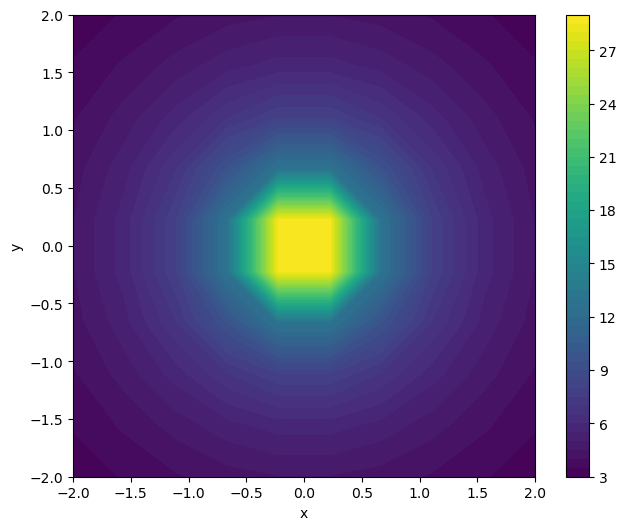
\includegraphics[width=0.35\textwidth]{papers/maxwell/skalar}}
	\subfigure{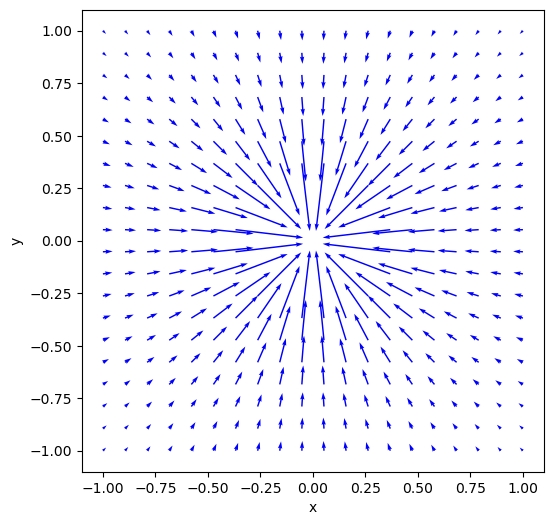
\includegraphics[width=0.3\textwidth]{papers/maxwell/gradient}}
	\caption{Skalar- und Vektorfeld}
	\label{maxwell:skalarGrad}
\end{figure}

\subsection{Vektorfeld\label{maxwell:vektorfeld}}

Ein Vektorfeld ist eine Funktion der Form \[ f: \mathbb{R}^n \rightarrow \mathbb{R}^m, \] welche jedem Punkt im Raum einen Vektor zuweist. 
Die Richtung dieses Vektors gibt hierbei an, in welche Richtung der Fluss des Feldes an diesem Punkt geht, während der Betrag die Intensität repräsentiert.



Des weiteren spricht man von stationären Vektorfelder, wenn sie zeitunabhängig sind und von homogenen Vektorfelder, wenn die Richtung und der Betrag der Vektoren ortsunabhängig sind, also wenn jeder Vektor die gleiche Richtung und den gleichen Betrag haben.

\subsection{Operationen}

\subsubsection*{Gradient}

\subsubsection*{Divergenz}

\subsubsection*{Rotation}

